\documentclass[10pt,article]{IEEEtran}

\usepackage{hyperref}
\usepackage{graphicx}	% For figure environment
\usepackage{enumitem}
\usepackage{lipsum}
\usepackage{booktabs}
\usepackage{tabularx}
\usepackage{adjustbox}
\usepackage[compact]{titlesec}
\usepackage{placeins}

\begin{document}
\title{ML Project 1: spot the Higgs boson}

\author{
  Manuel Leone, Gabriele Macchi, Marco Vicentini\\
  \textit{Department of Computer Science, EPFL Lausanne, Switzerland}
}

\maketitle

\begin{abstract}
Machine Learning techniques are becoming increasingly popular nowadays and they are used in several and different fields of science.  These techniques are useful when we deal with complex and high dimensional datasets, which sometimes represent the output of scientific experiments. In this project we implement from scratch some of the most popular methods, applying them to a dataset from CERN, in order to solve a problem of binary classification.
\end{abstract}

\section{Introduction}

The aim of this project is to find the best binary classification method in order to distinguish signals of the Higgs Boson from the background noise and so to predict the correct label for each new observation. We used the CERN’s dataset which summarizes collision experiments; the raw dataset includes 250.000 labeled events with 30 features each. First of all we had to clean this huge amount of data via data cleaning and features selection, because a well done preprocessing is a fundamental step to obtain good results in a machine learning project. Then we proceeded with the implementations of the mandatory machine learning methods such as Linear Regression, Ridge Regression and Logistic Regression. For more informations about implementation and discussion of these algorithms see Sections~\ref{subsec:model-impl} and ~\ref{subsec:model-proc}.

\section{Models and methods}
\label{sec:models-methods}

Implementing good machine learning methods requires skills in the fields of data analysis and algorithm design. Understanding the real meaning behind the data is an important step to choose the right direction in the following implementations. On the other hand, the broad panorama of ML algorithms in literature provides several possible implementations, that if not well implemented could change dramatically the performance of the algorithms. Our analysis will focus on these two aspects, that in this case are theory physic and pure statistical approach.
Before getting inside the developing process, the reader is advised that the preliminary step performed is a \textbf{dataset division}. Indeed, in order to have an idea of the  goodness of fit and to compare the methods, the algorithms were trained on 80\% of the available dataset and tested on the remaining 20\%.

\subsection{Basic ML implementations}
\label{subsec:model-impl}
The implementation of the base methods consists of six well known Machine Learning algorithm such as Gradient Descent, Stochastic Gradient Descent, Least Squares, Ridge Regression, Logistic Regression and Regularized Logistic Regression. The null values of the dataset were initially filled with the median of the respective column. The first computation concerned the entire dataset considered as one. In the table below different hyperparameters and results of the respective methods are shown. The accuracy achieved is computed on our \textbf{ test set}. These results were not good enough, so we decided to move on with data processing, as described in the next section.

\begin{table}[h!]
\resizebox{\columnwidth}{!}{%
\centering
\begin{tabular}{|l|l|l|l|l|l|} 
\cline{2-5}
\multicolumn{1}{l|}{}    & \multicolumn{4}{l|}{Hyperparameters Used} & \multicolumn{1}{l}{}  \\ 
\hline
Methods                  & $\lambda$ & $\gamma$ & Degree & Max Iter      & Acc. \\ 
\hline
Gradient Descent         & /      & $10^{-6}$ &   1     &   2000         &  0.718   \\ 
\cline{1-1}
Stochastic GD            & /      & $10^{-7}$ & 1      & 1000         & 0.704    \\ 
\cline{1-1}
Least Squares            & /      &  /      & 1      & /              & 0.741   \\ 
\cline{1-1}
Ridge Regression         & $10^{-8}$ &  /      & 6      & /              &   0.766   \\ 
\cline{1-1}
Logistic Regression      & /      &  $10^{-10}$      & 1      & 10000           &   0.735   \\ 
\cline{1-1}
Reg. Logistic Regression &  $10^{-8}$    &   $10^{-10}$      & 1      & 10000           &            0.735           \\
\hline
\end{tabular}%
}
  \caption{Accuracies of the six algorithms without feature processing}
  \label{tab:firstresults}
\vspace{-0.5cm}
\end{table}

\subsection{Dataset analysis and preprocessing}

% \begin{figure}[tbp]
%   \centering
%   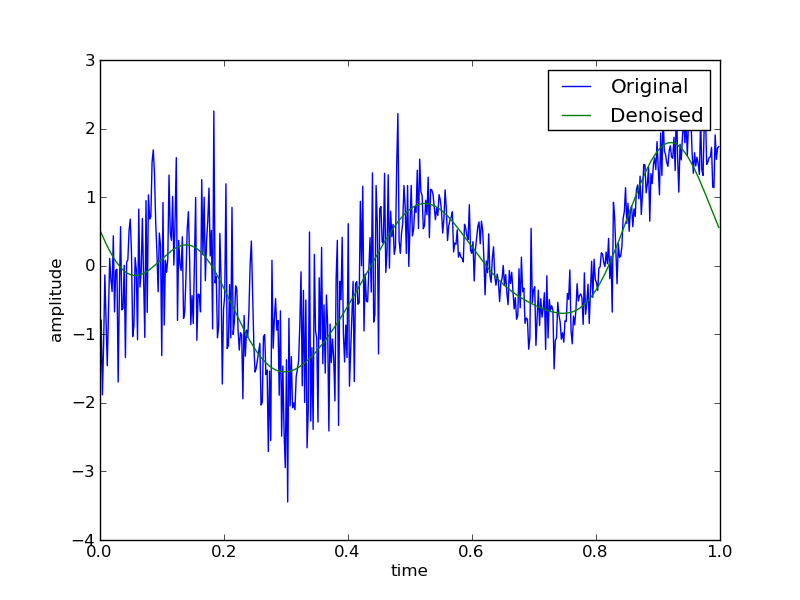
\includegraphics[width=\columnwidth]{denoised_signal_1d}
%   \caption{Signal compression and denoising using the Fourier basis.}
%   \vspace{-3mm}
%   \label{fig:denoise-fourier}
% \end{figure}
% \begin{figure}[htbp]
%   \centering
%   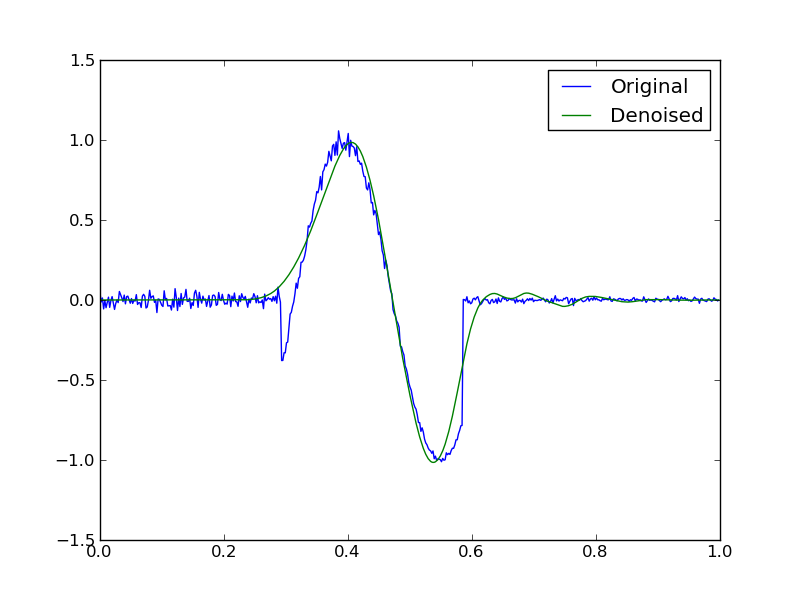
\includegraphics[width=\columnwidth]{local_wdenoised_1d}
%   \vspace{-3mm}
%   \caption{Signal compression and denoising using the Daubechies wavelet basis.}
%   \label{fig:denoise-wavelet}
% \end{figure}

% Use examples and illustrations to clarify ideas and results. For
% example, by comparing Figure~\ref{fig:denoise-fourier} and
% Figure~\ref{fig:denoise-wavelet}, we can see the two different
% situations where Fourier and wavelet basis perform well. 
The analysis of the dataset has been performed in different steps and each of them led to gradually improve the methods performances. The examinations we carried out are the following:
\subsubsection{NaN analysis} The official documentation \cite{higghsdoc} reports the dataset variables as either primitive (\texttt{PRI\_}), raw quantities directly measured from the collisions detector, or derived (\texttt{DER\_}), which are computed by the ATLAS physicist using the primitives. This information is useful to understand the physics meaning behind another fundamental fact: the dataset presents many -999.0 as placeholders for missing values. So, our first aim was to understand how we could impute these \textit{NaN}.\\
The analysis of the documentation shows a strict correlation between \textit{NaN} and the \texttt{PRI\_jet\_num} quantity. The jets are, from our understanding of the physic background, the sub particles produced in a collision. The main point to understand here is that some quantities are intentionally undefined because impossible to compute or no-sense with a number of jet equal to 0 or 1. With this cardinal concept in the head, we proceeded to a dataset categorization in four different subset based on the \texttt{PRI\_jet\_num}. As a result, we produced only columns totally full or totally empty from \textit{NaN} values, with the only exception of the \texttt{DER\_mass\_MMC} one.\\
At this point, we dropped all the columns totally filled with \textit{NaN} values. For the remaining missing elements we tried to use another time classical imputation methods such are using mean or median of the other values in the column. But this procedures never led us to a drastic gain in performance. Skilled by the experience of the previous division, we decided to carry out a second split for each of the 4 datasets based on \textit{NaN} remainings in \texttt{DER\_mass\_MMC}, producing a total of 8 subsets, now with no Null values at all.
\subsubsection{Correlation analysis} To better analyze each of the features we move further to plot the scatter matrix between all of them in all the subsets, in order to understand which of them have an high correlation or which are skewed. We discovered that at this point of the preprocessing pipeline some columns had the same values and a correlation of 1.00. We hypothesize that this features have the same physical meaning when considered only in the subset. To simplify our model and improve the prediction we decided do delete one of the two features.
\subsubsection{Skewness removal} The scatter plot matrix visualization pointed out the presence of many right-skewness distributions features. We applied cube root transformation to this columns to transform them into centered distributions.
\subsubsection{Adding 1s column and standardization} The last steps of the main preprocessing phase are data standardization followed by adding an all ones column. The former is performed to achieve better computation performance. The ones column precedes the feature matrix to be used as constant for the weights vector.
\subsubsection{Polynomial features} We proceeded to polynomial expansion of each subset by taking powers and stacking them together. A note on our polynomial implementation is that we perform the raising only from degree 1, as we already added an all ones column. The exact degree chosen via cross validation for each subset is presented in ~\ref{subsec:model-proc}.

\subsection{Model selection and processing}
\label{subsec:model-proc}
With our processed data, we can move to the second improvement task we have to perform: tuning the hyper-parameters of our best models.
We chose to dedicate our efforts only on Ridge Regression and Regularized Logistic Regression, as we saw at the very beginning of the project (TABLE ~\ref{tab:firstresults}), that the former outperforms the others, while the second should be the best for classification as for Machine Learning theory. We choose the Regularized version instead of the normal one to improve computational efficiency. For both of them we started by choosing the polynomial degree of all the subsets before moving on to the hyper-parameters selections.

For the Regularized Logistic Regression, we noticed almost immediately that using polynomial did not increase our performance sufficiently, so we decided to use only the first order degree. For the Ridge Regression our first tests pointed out an opposite situation, with a decreasing test loss by increasing the polynomial to a certain degree. 

After our previous tests, we performed a 12-fold cross-validation for the Ridge regression on our train set to choose the polynomial degree and the $\lambda$ parameter. For the Regularized Logistic Regression we could not do the same k-fold due to time constraints of the cross validation, so we tuned $\lambda$ and $\gamma$ with a simpler 4-fold cross-validation. The hyper-parameters best choices for both methods are shown in TABLE II.

\begin{table}[hbt]
\centering
\label{tab:hypersresults}
\resizebox{\columnwidth}{!}{%
\begin{tabular}{|c|c|l|l|l|}
\cline{2-5}
\multicolumn{1}{c|}{} & \multicolumn{2}{c|}{Ridge Regression} & \multicolumn{2}{c|}{Reg. Logistic Regression}  \\ 
\hline
Data-set              & degree & \multicolumn{1}{c|}{$\lambda$} & \multicolumn{1}{c|}{~ ~$\lambda $} & \multicolumn{1}{c|}{$\gamma$~ ~~} \\
\hline
Jet 0 without mass    & 7      & 2.4* $10^{-9}$    & $10^{-8}$     & $3.12*10^{-5}$             \\ 
\cline{1-1}
Jet 0 with mass       & 8      & $10^{-10}$        & $10^{-8}$     & $10^{-6}$                  \\ 
\cline{1-1}
Jet 1 without mass    & 5      & $4.89*10^{-10}$   & $10^{-8}$     & $3.12*10^{-5}$             \\ 
\cline{1-1}
Jet 1 with mass       & 8      & $5.30*10^{-9}$    & $10^{-8}$     & $10^{-6}$                  \\ 
\cline{1-1}
Jet 2 without mass    & 5      & $10^{-10}$        & $10^{-8}$     & $3.12*10^{-5}$             \\ 
\cline{1-1}
Jet 2 with mass       & 8      & $10^{-10}$        & $10^{-8}$     & $10^{-6}$                  \\ 
\cline{1-1}
Jet 3 without mass    & 2      & $10^{-10}$        & $10^{-8}$     & $10^{-3}$                  \\ 
\cline{1-1}
Jet 3 with mass       & 8      & $4.89 *10^{10}$   & $10^{-8}$     & $3.12*10^{-5}$             \\
\hline
\end{tabular}%
}
\caption{Hyper-parameters selection results}
\vspace{-0.5cm}
\end{table}
\FloatBarrier


\section{Results}
\label{sec:results}
The final results we achieved are computed with Ridge Regression and Regularized Logistic Regression using the 8-splitted dataset with no Nan, where the hyper-parameters and degrees are the ones obtained via cross validation. 

\begin{table}[!h]
\centering
\label{tab:finalresults}
\begin{tabular}{l|l|l|l}
\cline{2-3}
                                                 & Accuracy & F1-score          \\ 
\hline
\multicolumn{1}{|l|}{Ridge Regression}                     & 0.824     & 0.733             \\ 
\cline{1-1}
\multicolumn{1}{|l|}{Reg. Logistic Regression}  & 0.728          & 0.579                 \\
\hline
\end{tabular}
\caption{Final results for Ridge and Regularized Logistic Regression }
\vspace{-0.5cm}
\end{table}

From the theory we expected the results of Regularized Logistic Regression to be better than the one of the Ridge Regression, but maybe this was not the case for this particular problem or we did not manage to find the right hyper-parameters which led to this condition.


\section{Summary}

Overall, we can would conclude we are sufficiently satisfied of the results we achieved with our implementation, in particular if we consider that we just used basic machine learning tools. Anyway improving the accuracy is possible, but it would require extra time both in data analysis and hyper-parameters tuning. 

We learnt how preprocessing is crucial when dealing with Machine Learning implementation. We could have increased the goodness of the result by using optimal methods to clean our dataset or by adding important features, as example by performing cross-terms expansions. We also think that the presence of an expert in the topics we were dealing with would be helpful too. It this way we could have performed a better selection of the features based on deeper and insightful knowledge. It is also true, that the implementation of more advanced methods such as Neural Network or random forests would have helped us in reaching higher values of accuracy.


\bibliographystyle{IEEEtran}
\bibliography{literature}

\end{document}
